\chapter{Análisis y experimentación} \label{chap:analisis-y-experimentacion}

Una vez adquiridos los conocimientos teóricos necesarios, y comprendido el funcionamiento de los diferentes algoritmos que vamos a utilizar, estamos en disposición de aplicarlos a los datos de experimentación y comprobar la eficacia de los algoritmos en un caso real. Este capítulo aborda el trabajo realizado durante tres meses de prácticas en el Instituto Cajal, aplicando diferentes técnicas para tratar de agrupar los comportamientos de los animales, y de diferenciar animales bajo efectos de tratamiento o de placebo.

En la Sección \ref{sec:preprocesado} tratamos como hemos preprocesado los videos para homogeneizar todas las sesiones de experimentación, obtener los datos de posición de los animales en ellas y filtrar e interpolar los datos poco verosímiles. En la Sección \ref{sec:análisis} desarrollamos el proceso de análisis de los datos preprocesados aplicando los diferentes algoritmos vistos anteriormente y analizando sus resultados.

\section{Preprocesado de datos} \label{sec:preprocesado}

Los datos de los que hemos partido para realizar el análisis han sido 88 pares de videos en blanco y negro, de unos cinco minutos cada uno, de ratones en su caja sin estar realizando ninguna tarea concreta. Cada par de videos consistía en un video de la vista cenital de la caja y otro de la vista lateral, como se puede observar en la Figura \ref{fig:deeplabcut-outputexamples}. Además, de cada par de videos teníamos el código del animal que estaba siendo grabado, la fecha de la sesión y si el animal estaba bajo los efectos del tratamiento de NDMA en dicha fecha o no. Mostramos un resumen de estos datos en la Tabla \ref{tab:animal-info}.

% Animal info
\begin{table}[h]
  \centering
  \begin{tabular}{|c|c|c|c|}
    \hline
    \textbf{Video} & \textbf{Código del animal} & \textbf{Fecha de la sesión} & \textbf{Tratamiento} \\ 
    \hline
    1 & 4128	& 2020-12-02	& CONTROL \\ 	
    2 & 4128	& 2020-11-21	& CONTROL \\ 	
    3 & 4128	& 2020-11-23	& CONTROL \\ 
    ... &  ...	& ... & ... \\ 
    80 & 4108	& 2020-09-25	& NMDA	\\ 
    81 & 4089	& 2020-09-18	& NMDA	\\
    82 & 4089	& 2020-09-12	& CONTROL	\\ 
    83 & 4089	& 2020-09-24	& NMDA	\\
    \hline
  \end{tabular}
  \caption[Datos de las sesiones]{Fragmento del \texttt{DataFrame} que almacenaba los datos de las sesiones, incluyendo el número del video según se almacenaban en memoria, el código del animal, la fecha de la sesión y el estado del tratamiento.}
  \label{tab:animal-info}
\end{table}

Para tratar de averiguar de forma automática el tipo de tratamiento de cada sesión, podríamos entrenar una red neuronal utilizando directamente los videos como datos de entrenamiento. Sin embargo, no contamos con una cantidad muy elevada de videos para entrenar, y además esto no nos daría ninguna pista sobre como comportamientos concretos se relacionan con el tratamiento. Al no contar con una base de datos de fragmentos de videos clasificados según el comportamiento del animal, tampoco podemos entrenar una red para distinguir estos comportamientos sin tener que pasar antes por un seguramente tedioso periodo de etiquetado manual de fragmentos. Por ello, hemos hecho uso de la herramienta DeepLabCut para rastrear la posición del ratón en cada fotograma y así poder hacer cálculos sobre ella, y trabajar con otros algoritmos de agrupación no supervisada para tratar de clasificar diferentes movimientos del ratón a lo largo del video.

\subsection{DeepLabCut}\label{sec:DeepLabCut}

(EXPLICACIÓN DEEPLABCUT)

% DeepLabCut output
\begin{figure}[]
  \centering
  \begin{subfigure}{0.45\textwidth}
    \centering
    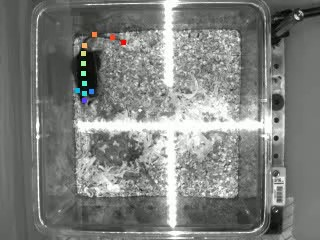
\includegraphics[width=\textwidth, angle=-90]{figures/deeplabcut-top-example-4128-2020-12-02-1-00-37.jpg}
    \caption{}
    \label{fig:deeplabcut-top-example}
  \end{subfigure}
  \begin{subfigure}{0.45\textwidth}
    \centering
    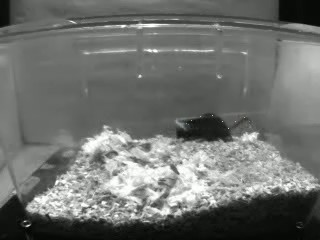
\includegraphics[width=\textwidth]{figures/deeplabcut-lateral-example-4128-2020-12-02-1-00-37.jpg}
    \caption{}
    \label{fig:deeplabcut-lateral-example}
  \end{subfigure}
  \begin{subfigure}{0.45\textwidth}
    \centering
    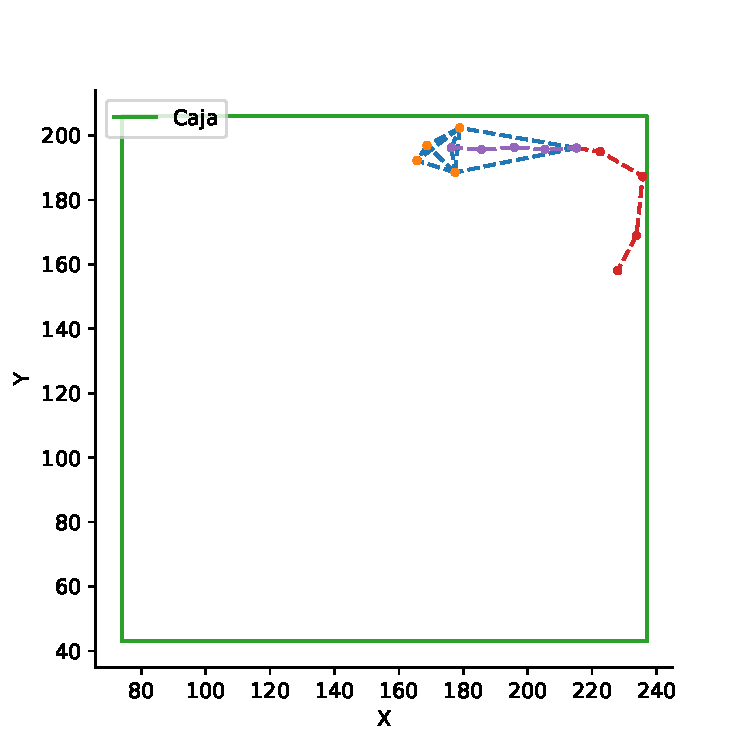
\includegraphics[width=\textwidth]{figures/triangulation-top-4128-2020-12-02.pdf}
    \caption{}
    \label{fig:triangulation-top}
  \end{subfigure}
  \begin{subfigure}{0.45\textwidth}
    \centering
    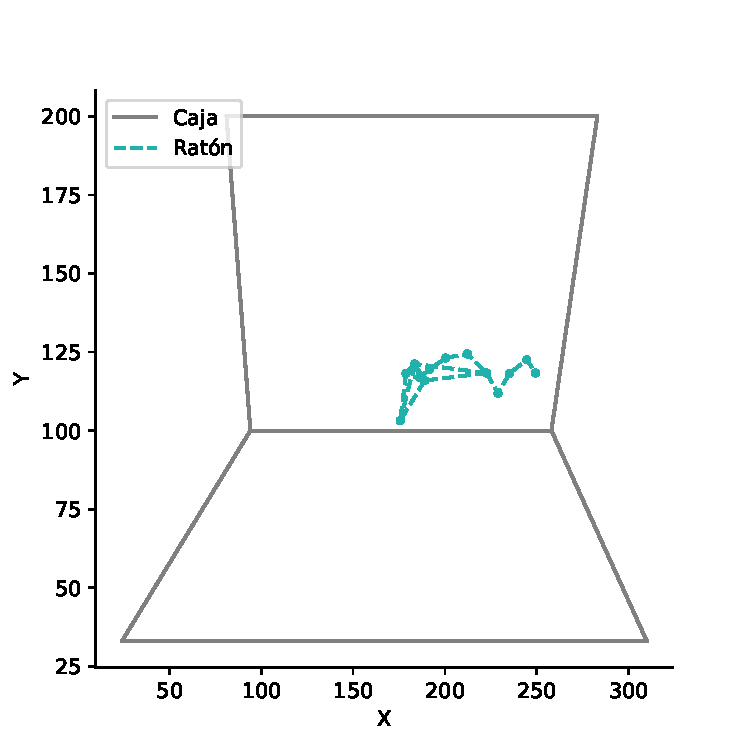
\includegraphics[width=\textwidth]{figures/triangulation-lateral-4128-2020-12-02.pdf}
    \caption{}
    \label{fig:triangulation-lateral}
  \end{subfigure}
  \caption[Salida de DeepLabCut.]
  {Salida de DeepLabCut del animal 4128 el 02-12-2020, 1:00:37. \ref{fig:deeplabcut-top-example} Video de la vista cenital de la caja. Los puntos sobre el animal son los dibujados por DeepLabCut para rastrear las partes del animal. \ref{fig:deeplabcut-lateral-example} Video de la vista lateral de la caja. \ref{fig:triangulation-top} En azul, la triangulación formada por los puntos obtenidos por DeepLabCut de la vista cenital. Cinco puntos para la cabeza, cuatro para la espalda y otros cuatro para la cola. En gris, las dimensiones de la base de la caja, obtenidas midiendo las distancias en píxeles sobre un fotograma de video. \ref{fig:triangulation-lateral} Análogo a la vista cenital, desde la vista lateral. En gris, la altura mínima del suelo de la caja y su pared trasera.}

  \label{fig:deeplabcut-outputexamples}
\end{figure}

% Dataframe example
\begin{table}[h]
  \centering
  \begin{tabular}{|c|c|c|c|c|c|c|}
  \hline
    & Nosex & Nosey & Noselikelihood & Headx & Heady & ... \\
  \hline
  0 & 136.165344 & 177.722496 & 0.000084 & 129.790253 & 174.772552 & ... \\
  1 & 162.032005 & 201.444756 & 0.942181 & 168.152061 & 202.420639 & ... \\
  2 & 156.297043 & 200.326378 & 0.000073 & 162.436028 & 203.156837 & ... \\
  3 & 155.370415 & 199.043297 & 0.000277 & 159.507599 & 200.199928 & ... \\
  4 & 149.272644 & 197.677170 & 0.000045 & 155.493912 & 198.814835 & ... \\
  ... & ... & ... & ... & ... & ... & ... \\
  \hline
  \end{tabular}
  \caption[Datos de DeepLabCut]{Extracto del \texttt{DataFrame} de \texttt{pandas} de los datos sin procesar de DeepLabCut. Para cada punto rastreado, y para cada fotograma del video, se computa la predicción de la coordenada $x$ y de la coordenada $y$ y se da la verosimilitud de dicha predicción.}
  \label{tab:df-example}
\end{table}

\subsection{Filtrado e interpolación}
Una vez hemos pasado todos los videos por DeepLabCut, tenemos dos ficheros de datos para cada uno de las sesiones, uno para las coordenadas de los puntos de la vista cenital y otro para las coordenadas de los puntos de la vista lateral. Al cargar los ficheros a memoria como \texttt{DataFrames} de \texttt{pandas}, vemos que no todos ellos tienen la misma duración, por lo que los homogeneizamos todos eliminando los datos de los últimos fotogramas, consiguiendo que cada \texttt{DataFrame} tenga un tamaño de 6000 filas, lo que equivale a 6000 fotogramas o 5 minutos de video. Además, eliminamos los datos de 4 videos que no llegan a esa duración, ya que son videos con problemas que no entorpecerían el análisis. Uno de ellos solo duraba 3 minutos ya estaba mal grabado y al final estaba a cámara rápida, por ejemplo.


% Raw trayectory
\begin{figure}[]
  \centering
  \begin{subfigure}{0.45\textwidth}
    \centering
    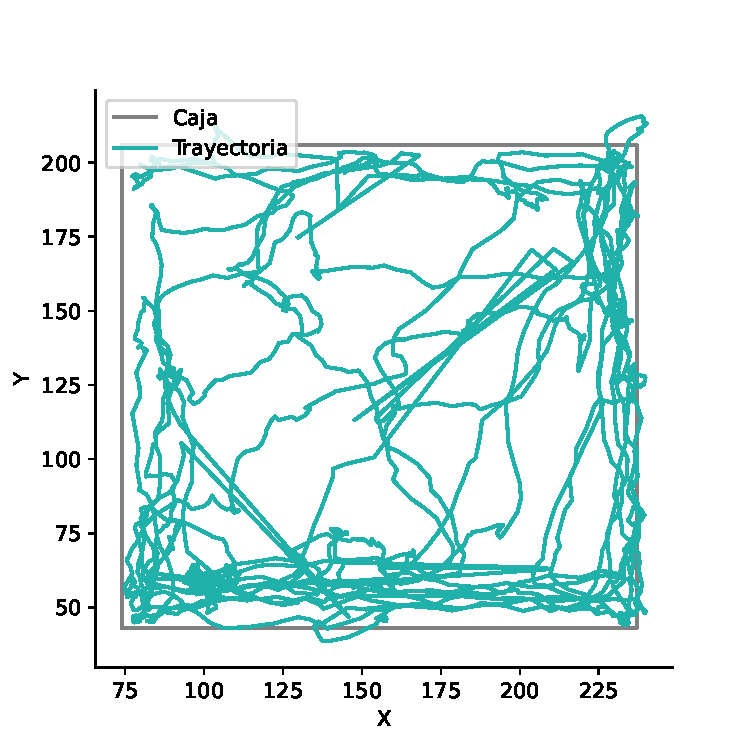
\includegraphics[width=\textwidth]{figures/raw-trayectory-top-4128-2020-12-02.pdf}
    \caption{}
  \end{subfigure}
  \begin{subfigure}{0.45\textwidth}
    \centering
    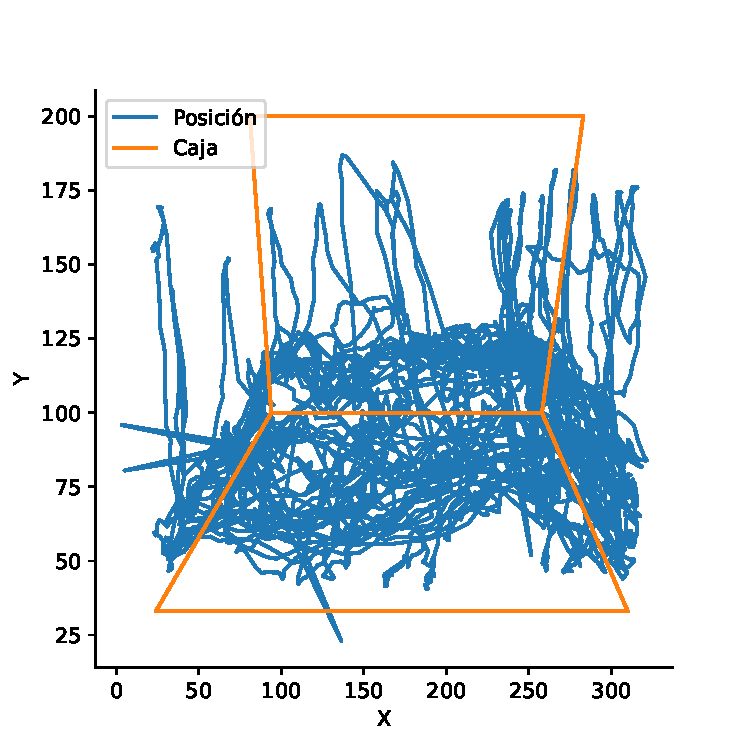
\includegraphics[width=\textwidth]{figures/raw-trayectory-lateral-4128-2020-12-02.pdf}
    \caption{}
    \label{fig:raw-top}
  \end{subfigure}
  \begin{subfigure}{0.45\textwidth}
    \centering
    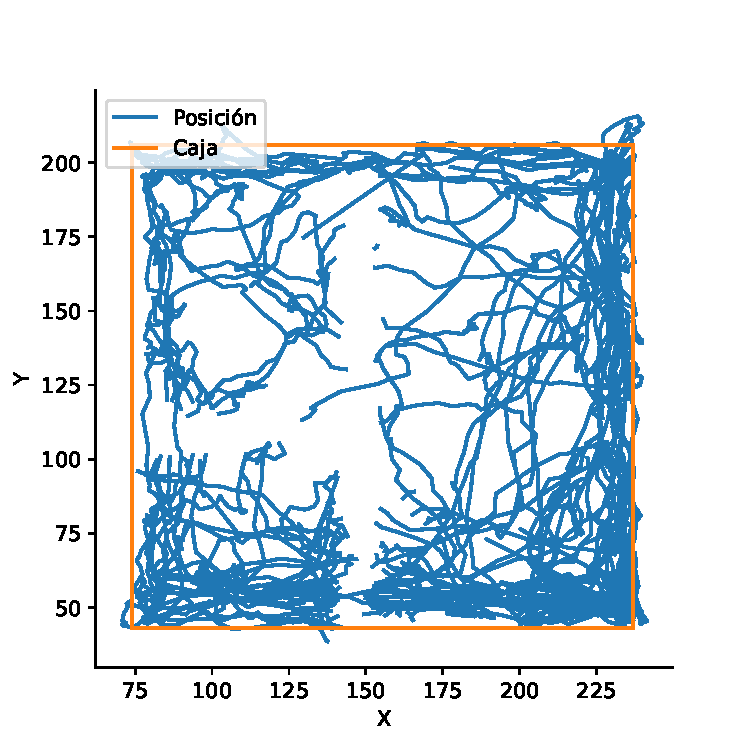
\includegraphics[width=\textwidth]{figures/filtered-trayectory-top-4128-2020-12-02.pdf}
    \caption{}
  \end{subfigure}
  \begin{subfigure}{0.45\textwidth}
    \centering
    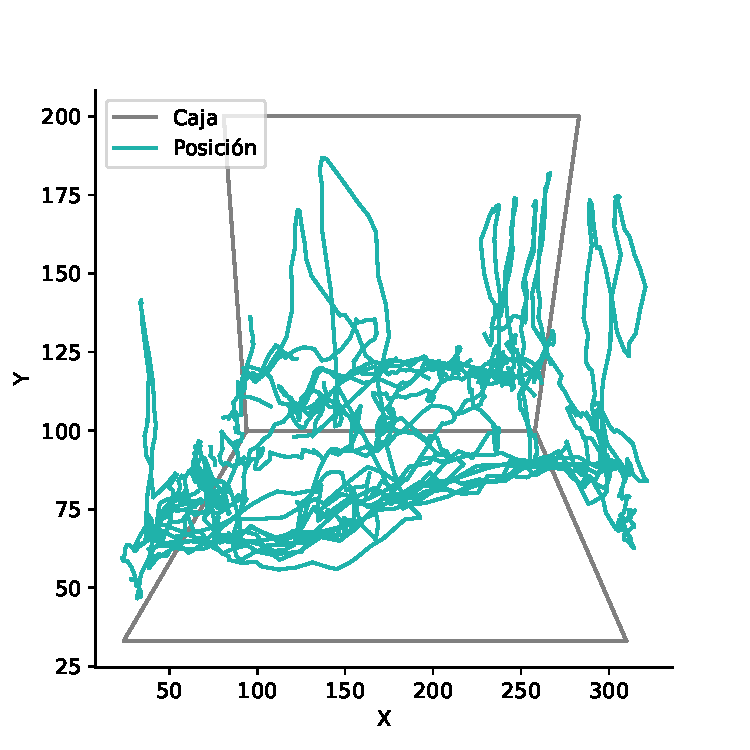
\includegraphics[width=\textwidth]{figures/filtered-trayectory-lateral-4128-2020-12-02.pdf}
    \caption{}
  \end{subfigure}
  \caption[Trayectorias durante el preprocesado.]{Vistas cenital y lateral de trayectorias de un punto de la cabeza del animal. Datos correspondientes a los dos primeros minutos de la sesión del 2020-12-02 del animal 4128. \ref{fig:raw-top}: Vista cenital de los datos antes del preprocesado. En gris se ha dibujado las dimensiones de la caja y en color la trayectoria del punto \texttt{Head}.}
  \label{fig:raw-trayectories}
\end{figure}

\begin{figure}[]
  \centering
  \begin{subfigure}{0.45\textwidth}
    \centering
    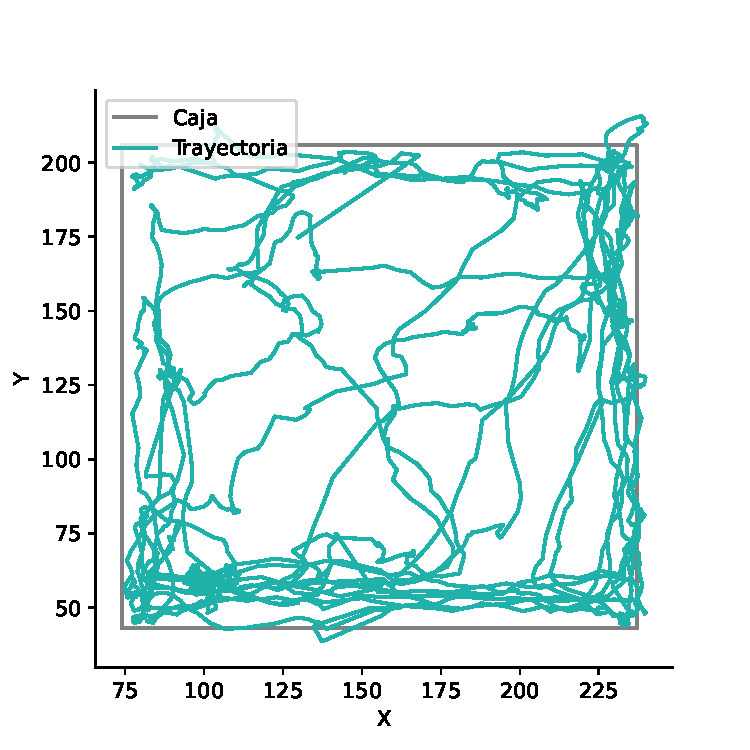
\includegraphics[width=\textwidth]{figures/interpolated-trayectory-top-4128-2020-12-02.pdf}
    \caption{}
    \label{fig:inter-top}
  \end{subfigure}
  \begin{subfigure}{0.45\textwidth}
    \centering
    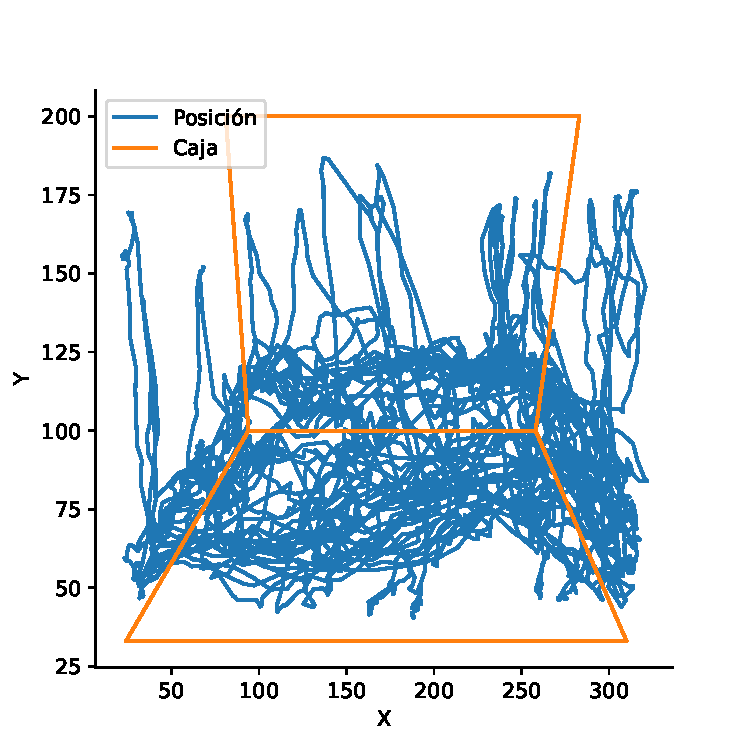
\includegraphics[width=\textwidth]{figures/interpolated-trayectory-lateral-4128-2020-12-02.pdf}
    \caption{}
    \label{fig:inter-lateral}
  \end{subfigure}
  \caption[Trayectorias preprocesadas.]{Vistas cenital y lateral de trayectorias de un punto de la cabeza del animal. Datos correspondientes a los dos primeros minutos de la sesión del 2020-12-02 del animal 4128. \ref{fig:inter-top}: Vista cenital de los datos filtrados e interpolados. En gris se ha dibujado las dimensiones de la caja y en color la trayectoria del punto \texttt{Head}.}
  \label{fig:interpolated-trayectories}
\end{figure}


\subsection{Computo de variables a analizar}

Una vez todos los datos han sido preprocessados, podemos computar diferentes propiedades de los mismos para usarlas posteriormente en los algoritmos de agrupación o de reducción de dimensiones. Además, podemos computar puntos de mayor confianza calculando medias de otros puntos individuales.

(FINALIZAR SECCIÓN e INCLUIR FIGURAS)

\blankpage
\section{Análisis de datos} \label{sec:análisis}

\subsection{Agrupaciones respecto a la trayectoria.}
(Explicar como se han fragmentado los videos para tratar de realizar agrupaciones de que está haciendo el animal en cada momento y para tratar de si se trata de un animal bajo los efectos del tratamiento o no.)

\subsection{Agrupaciones incluyendo más variables computadas.}
(Mismo proceso que en la sección anterior pero ahora incluyendo mas variables además de la trayectoria, como velocidades, aceleración, angúlos...)

\subsection{Agrupamiento mediante una red neuronal.}
(Mismo procedimiento, pero ahora tratar de separar los dos tipos de animales entrenando una red neuronal.)